\newpage
\section{Nozioni introduttive}
La società moderna è una società digitale. Le immagini passano generalmente per un calcolatore prima di essere stampate, o in ogni caso possono essere sempre scannerizzate (con strumenti più o meno precisi) così da averne una copia digitale.
\`E in questa fase che l'immagine subisce il processo di filtraggio, nel calcolatore, quando è in formato digitale, Per capire cos'è un filtro occorre dunque chiedersi cosa sia un'immagine digitale.

\subsection{Immagini digitali}
\`E necessario comprendere a fondo cosa sia un oggetto, per poterlo poi implementare in un calcolatore, a tal scopo è utile quindi capire esattamente che cos'è un'immagine

\begin{quote}
\epigraph{\textit{Forma esteriore degli oggetti corporei, in quanto viene percepita attraverso il senso della vista, o si riflette – come realmente è, o variamente alterata – in uno specchio, nell’acqua e sim., o rimane impressa in una lastra o pellicola o carta fotografica.}}{Vocabolario Treccani}
\end{quote}

\noindent
Un'immagine viene rappresentata, impressa quindi su superfici, cioè oggetti bidimensionali, di dimensioni finite e le vediamo perchè i nostri occhi percepiscono il susseguirsi di colori diversi. Come codificare tali entità?
Come per tutti gli oggetti reali, sebbene abbiano dimensioni finite, le immagini sono distruibuzioni continue, o per meglio dire, il susseguirsi delle gradazioni di colore avviene in una maniera che possiamo considerare come continua. Questo è il primo problema che ci si pone quando si pensa a come codificare delle immagini.\\
La soluzione più largamente utilizzata è anche quella più semplice ed intuitiva, ossia di discretizzare tale distribuzione di colori. Si divide l'immagine con una griglia e ad ogni casella, che d'ora in poi chiameremo \textbf{pixel}, assegnamo un colore.
\`E ovvio che così facendo si perdono dei dettagli, la quantità di dettagli che riusciamo a conservare può variare enormemente, una minima quantità di dettagli si perde sempre ma è un prezzo che vale la pena pagare.
\newpage
Facciamo un esempio:

%\ref{fig:figuraa}. 
\begin{figure}[htb] \centering
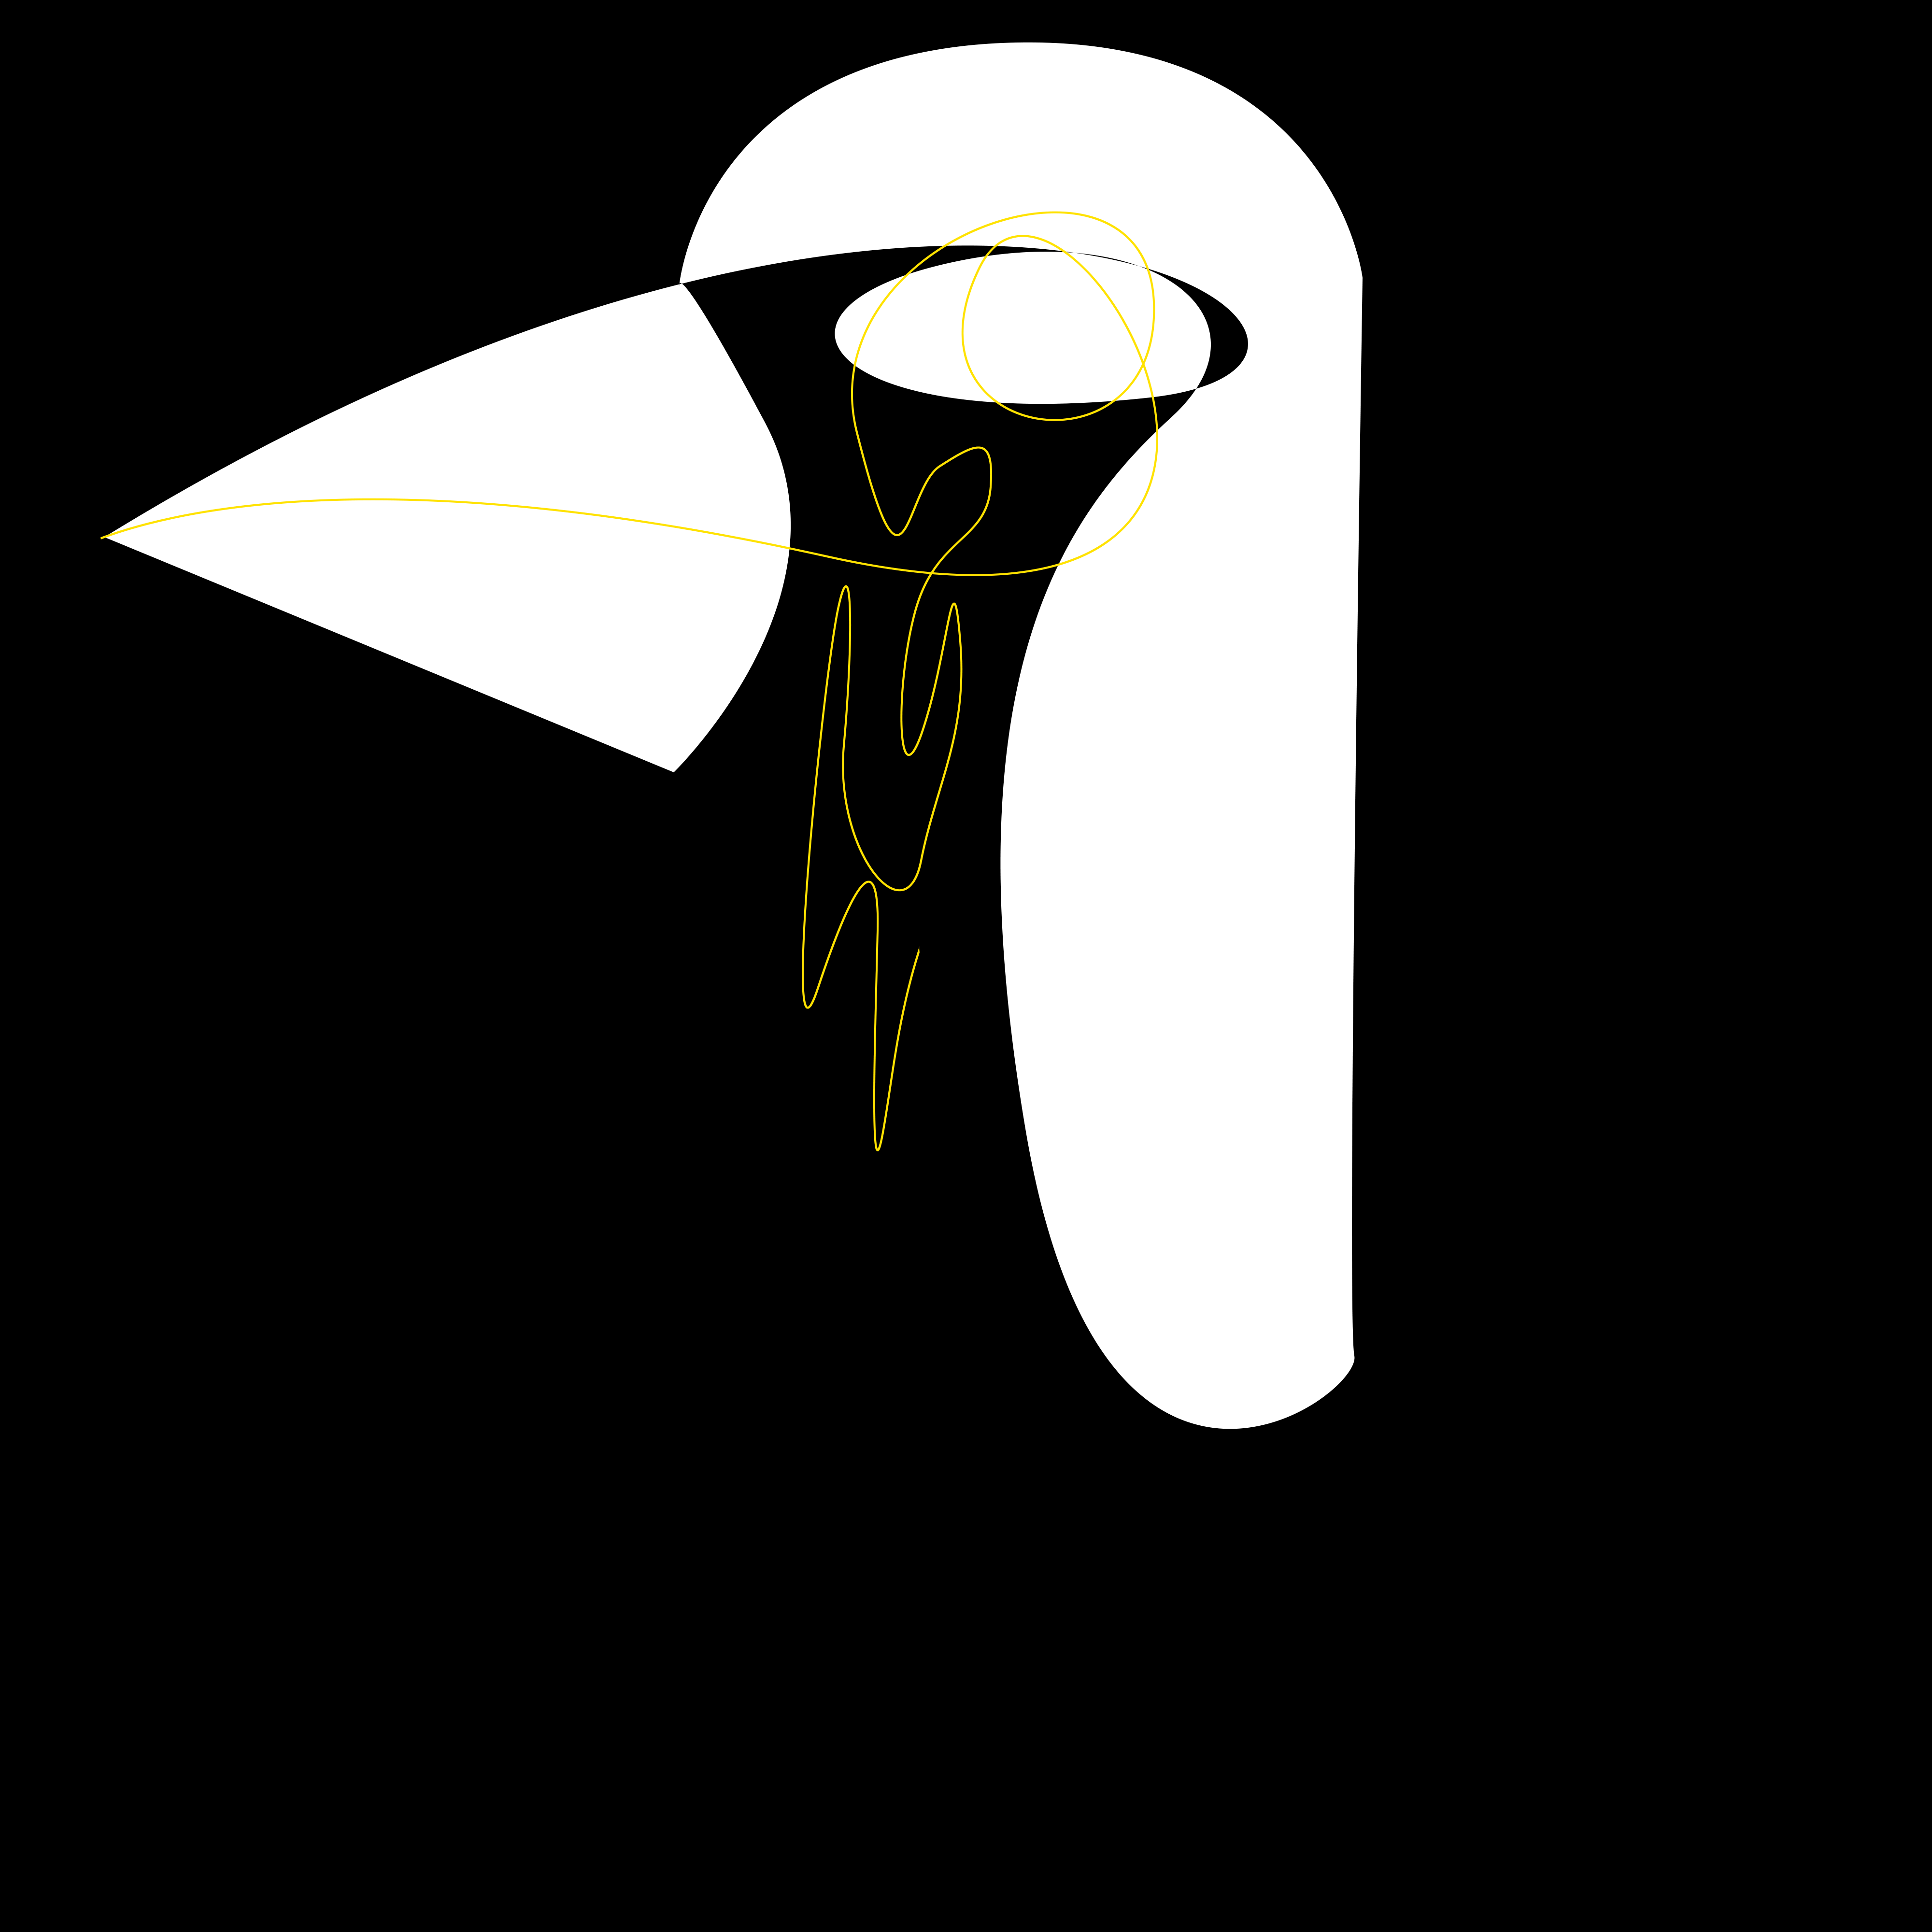
\includegraphics[scale=0.08]{Pictures/in ricordo del pinguino cameriere.png}
%\caption{Fiamme.}\label{fig:figura}
\qquad\qquad

\includegraphics[scale=0.08]{Pictures/canvas8x8.png}
\caption{Confronto tra immagine originale e immagine codificata utilizzando una griglia 4x4.}\label{fig:figura}
\end{figure}

%\ref{fig:figura}. 
\begin{figure}[htb] \centering
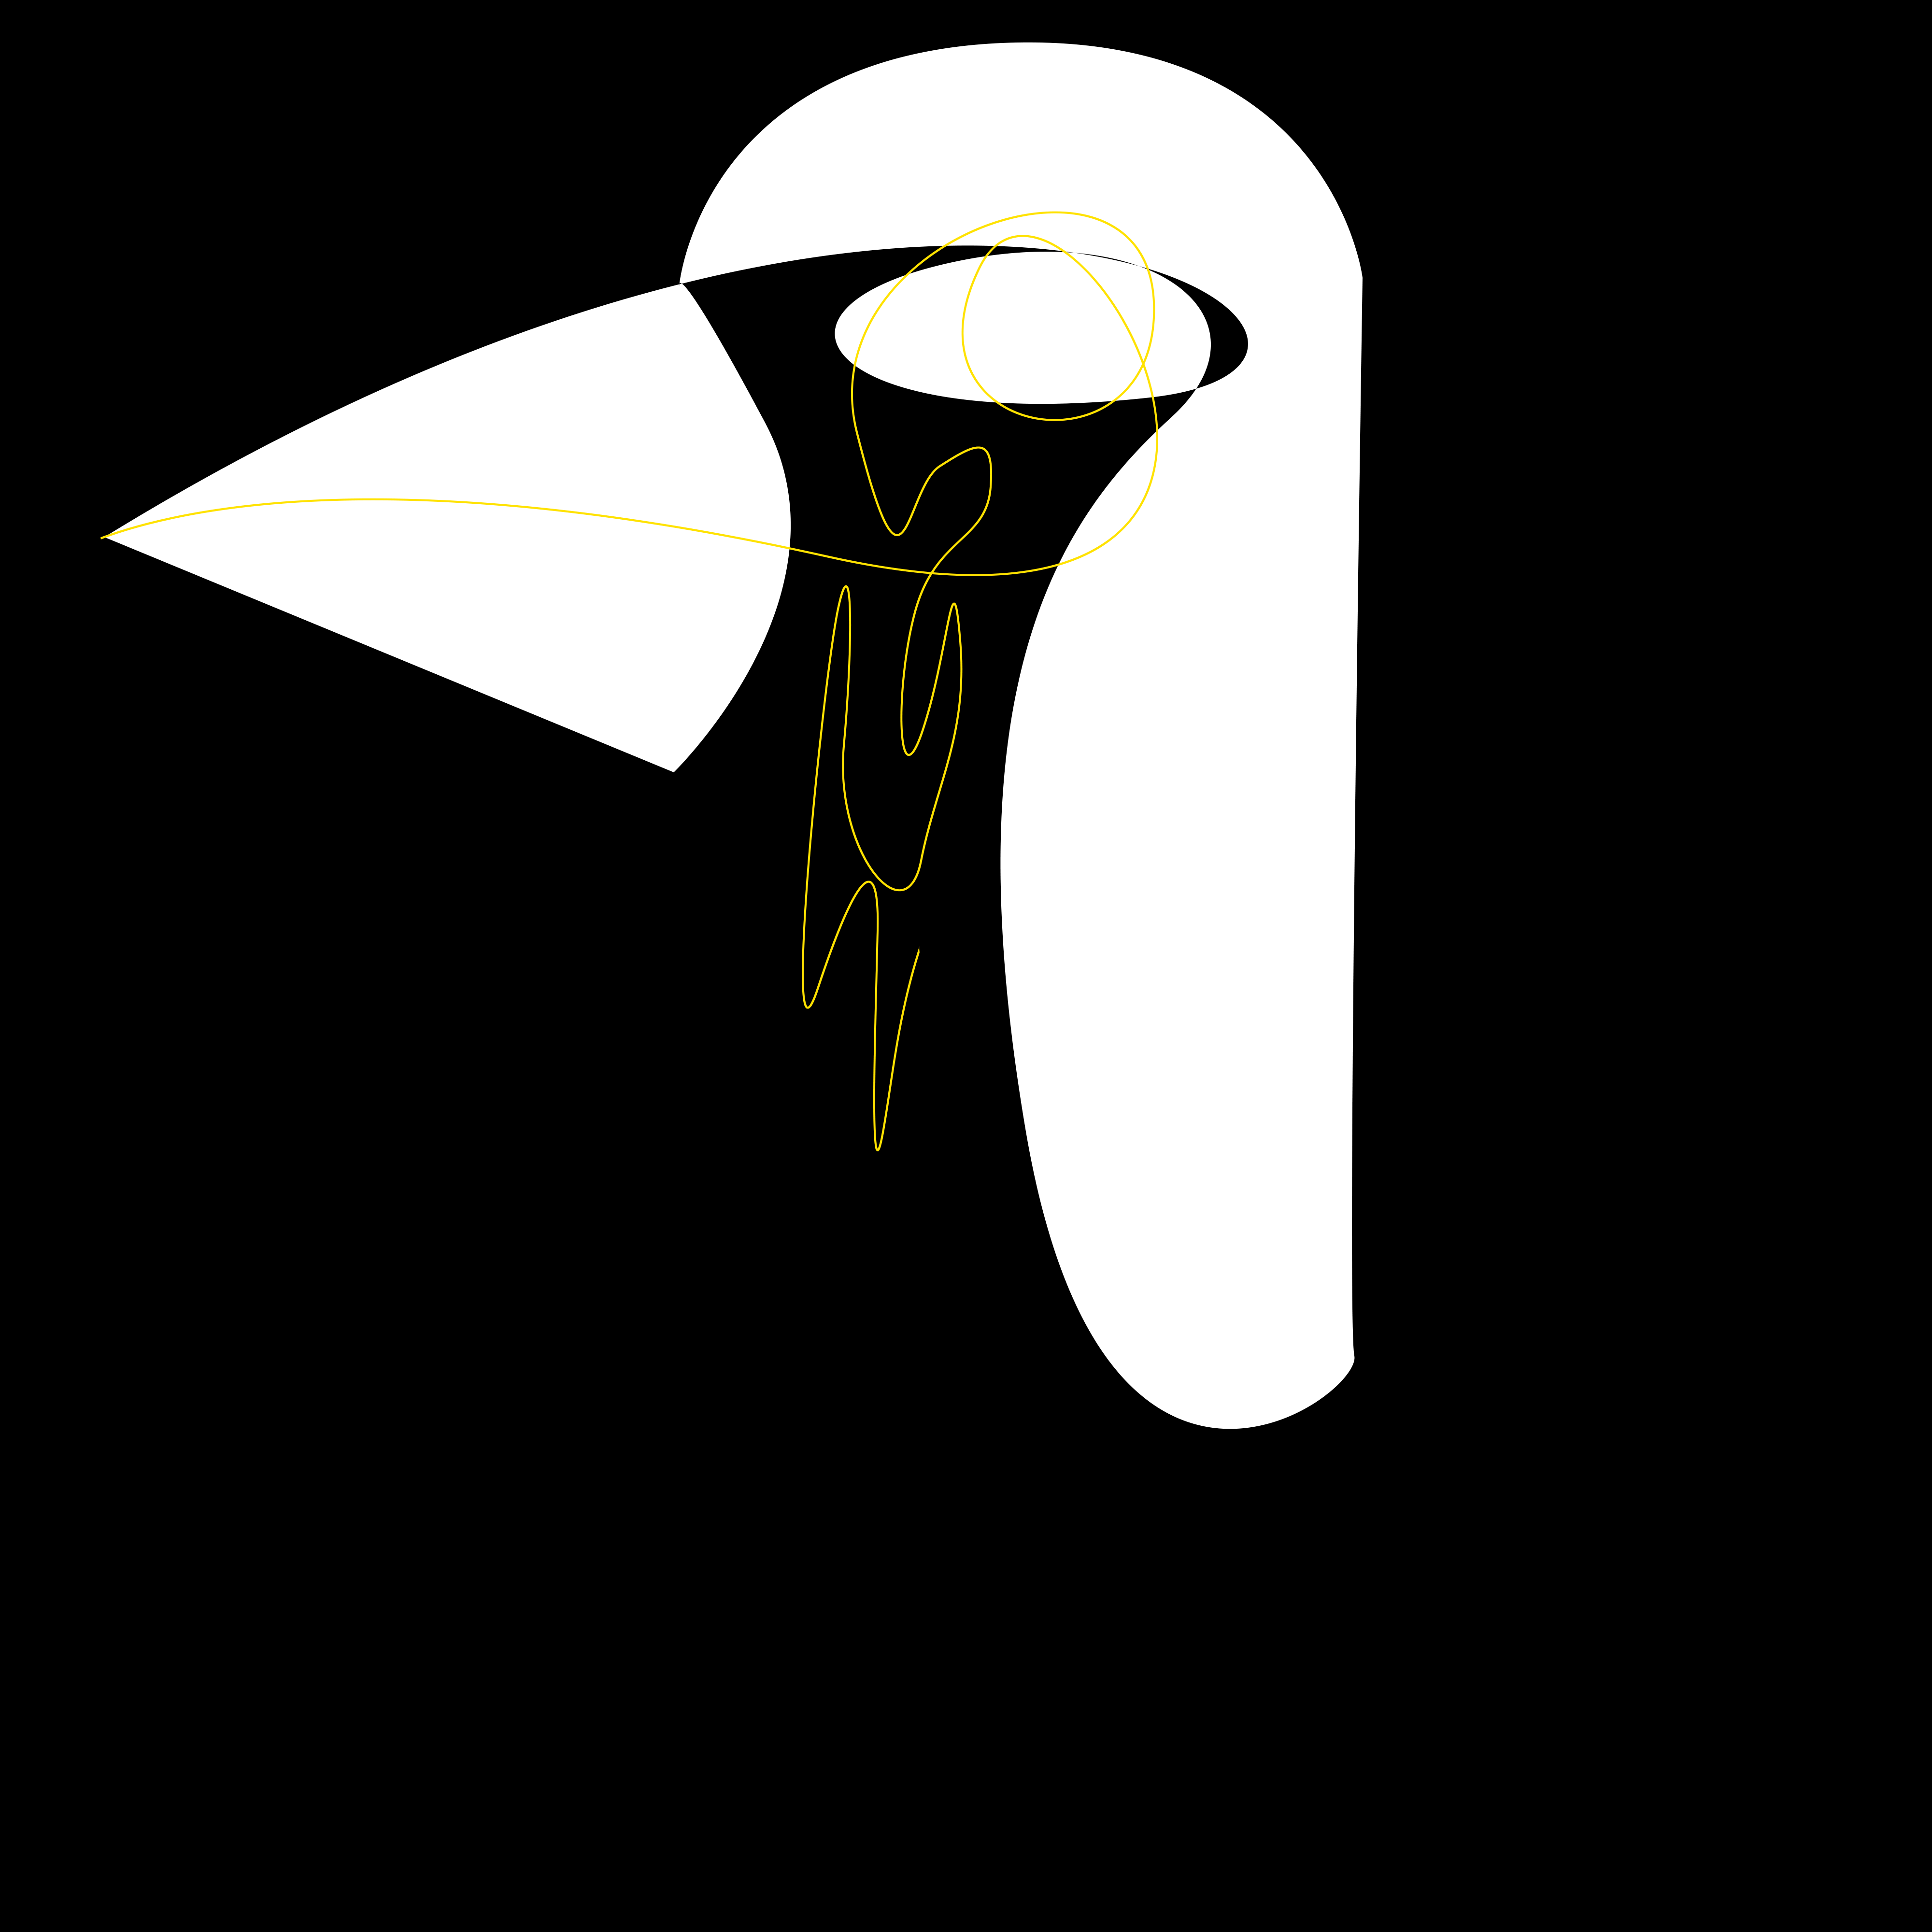
\includegraphics[scale=0.08]{Pictures/in ricordo del pinguino cameriere.png}
\qquad\qquad
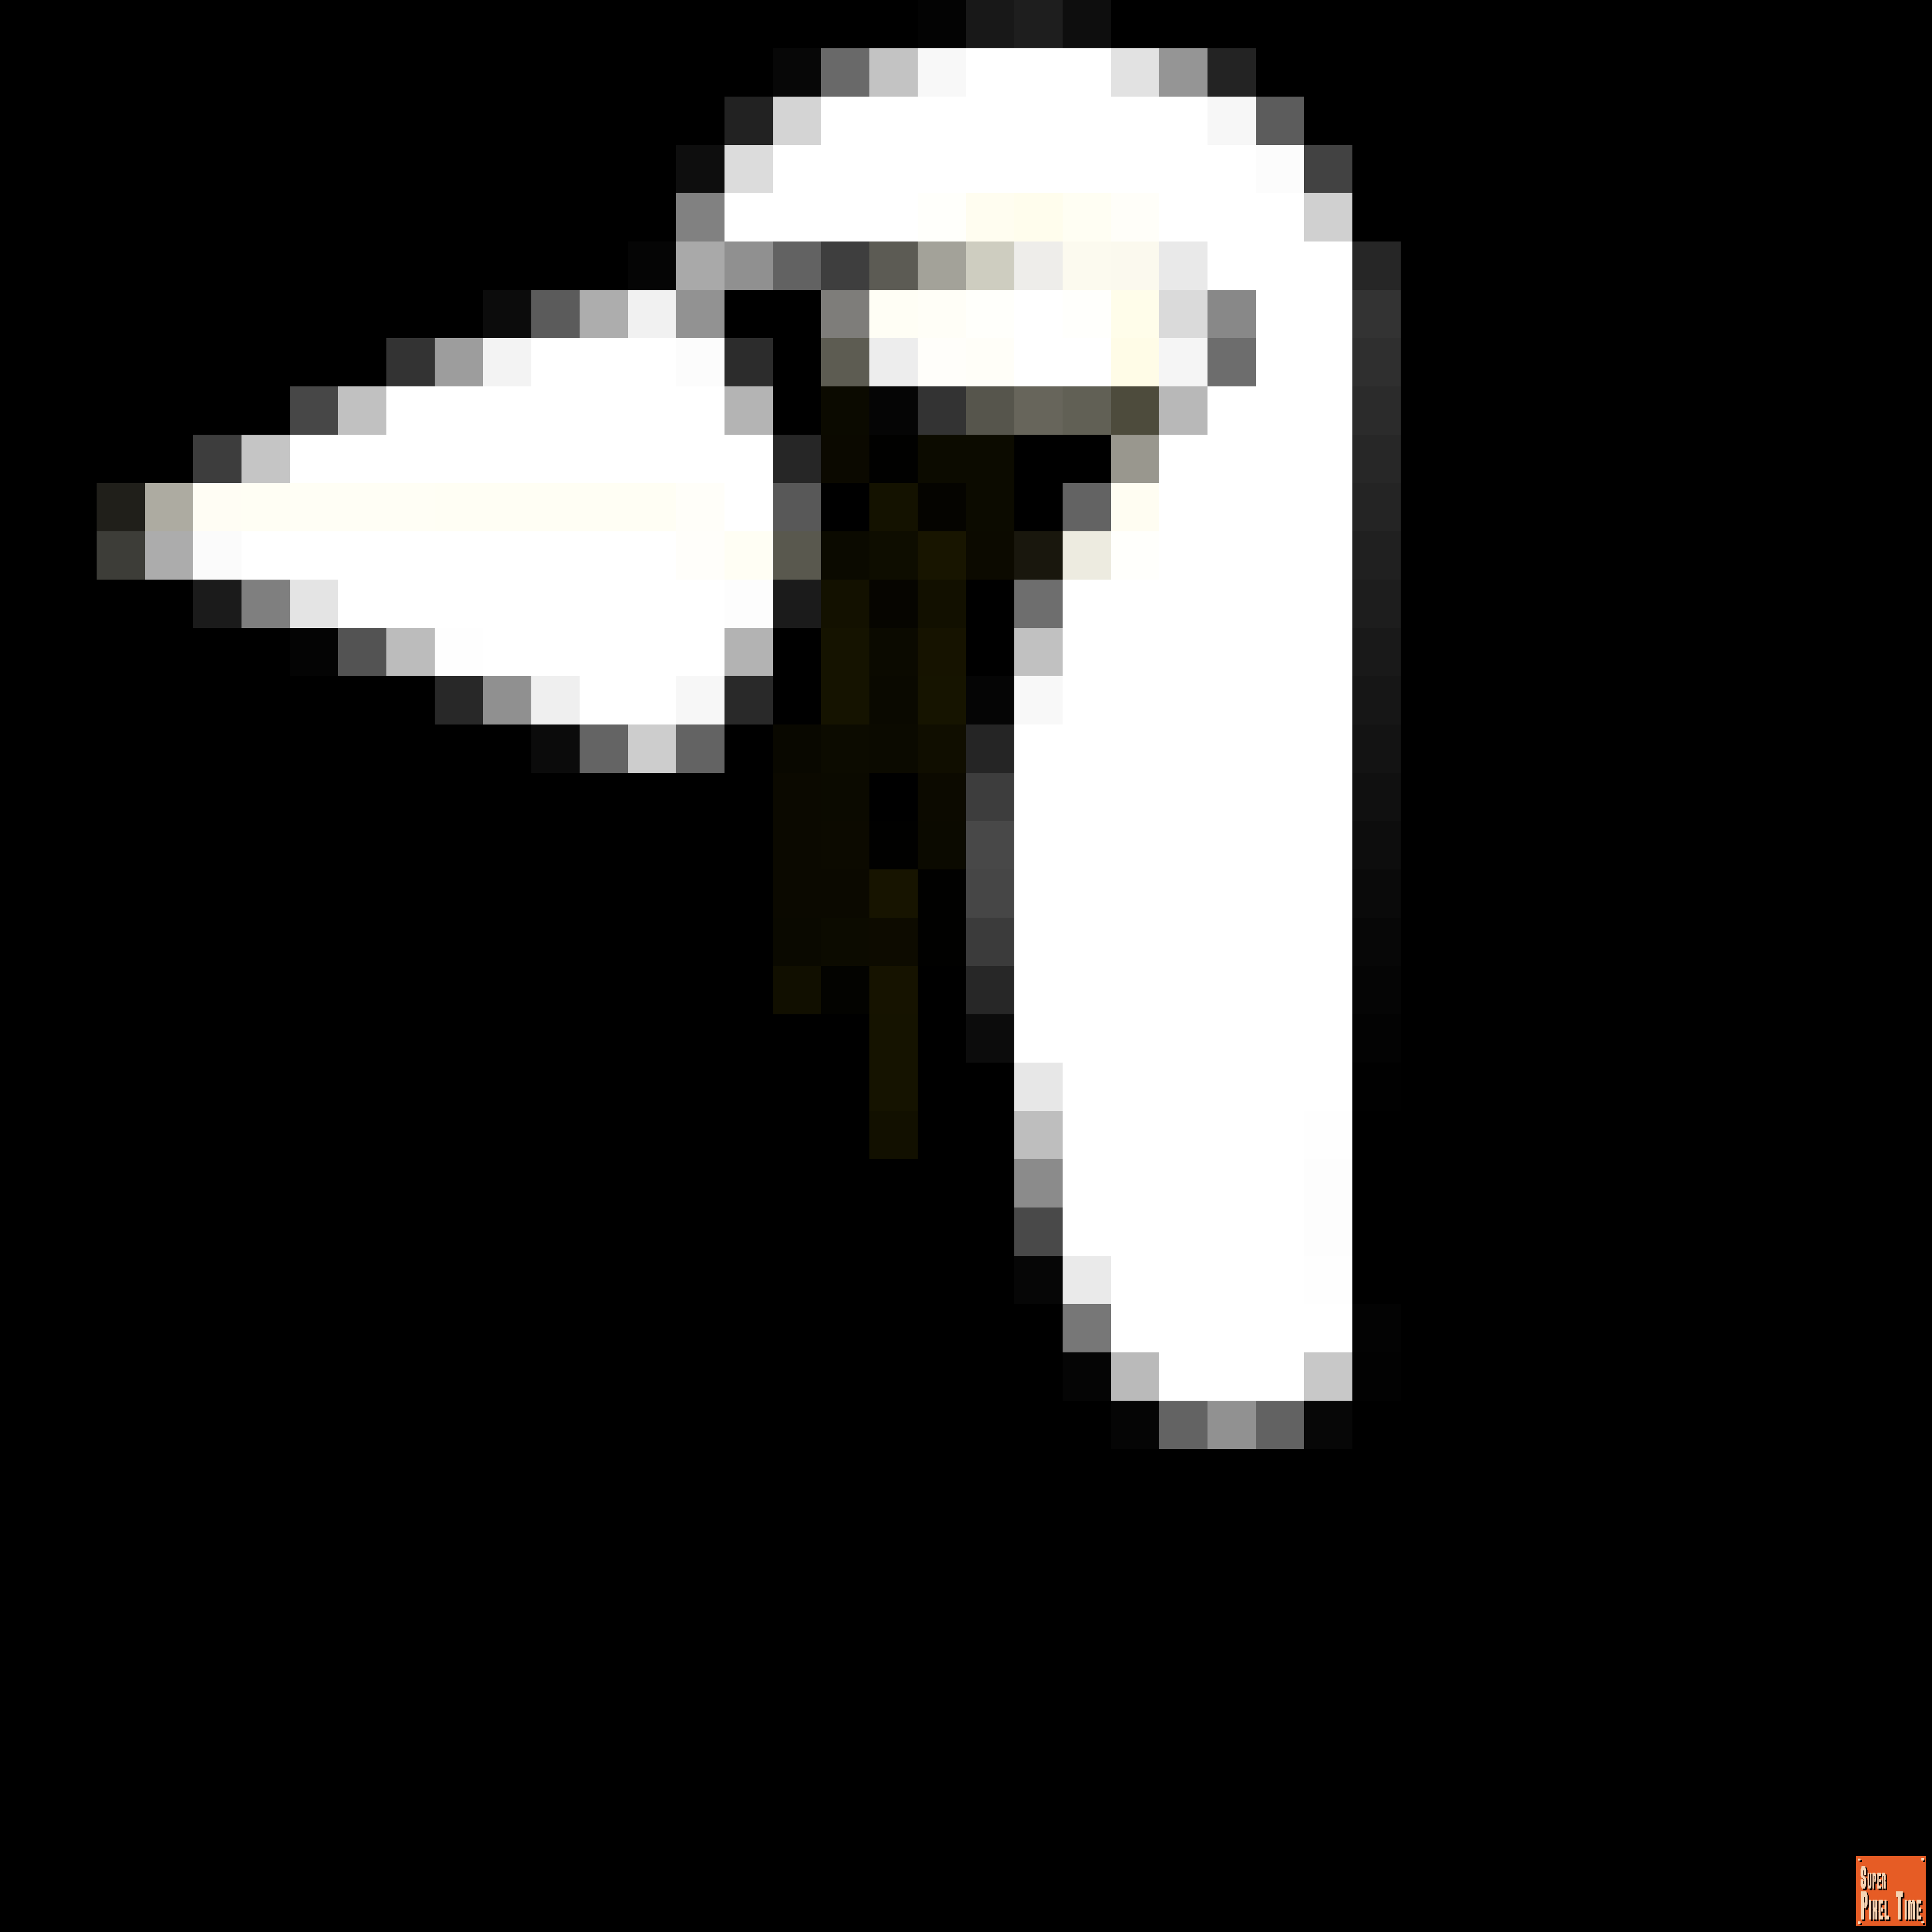
\includegraphics[scale=0.08]{Pictures/canvas80x80.png}
\caption{Confronto tra immagine originale e immagine codificata utilizzando una griglia 80x80.}\label{fig:figura}
\end{figure}

\noindent
\`E semplice vedere come ad una griglia più fitta corrisponda una miglior qualità dell'immagine, questo è il concetto di \textbf{risoluzione di un'immagine}. 
Una miglior risoluzione però costa, come anticipato, in termini di memoria. Una griglia 4x4 corrisponde a 16 pixel, ad una griglia 80x80 corrispondono invece 6400 pixel! Questo vuol dire che la seconda immagine pesa 400 volte di più della prima.

\vspace{1em} \noindent
Volendo definire in maniera più precisa che cosa è un'immagine digitale, diremmo che quest'ultima è una funzione da $\mathbb R^2$ in $\mathbb R^3$ cioè, date in input due coordinate, essa restituisce un colore (che è formato da 3 canali RGB). Se però l'immagine è in bianco e nero la questione si semplifica: l'immagine diventa una funzione da $\mathbb R^2$ in $\mathbb R$, dal momento che per codificare un colore appartenente alla scala di grigio basta un solo canale: il livello di luminosità. Difatti, la riduzione da tre ad un solo canale rappresenta un grosso vantaggio, permettendo di diminuire di due terzi lo spazio di memoria occupato.

\subsection{Cosa sono i filtri}
Una volta capito che un'immagine è una funzione possiamo definire un filtro come una seconda funzione che convoluta alla prima da il risultato richiesto.\\
Una equazione alle derivate parziali (PDE) esprime una evoluzione. Sia u la nostra immagine e $u_0$ lo stato in cui si trova inzialmente, allora per convoluzione possiamo dire che 

\begin{equation} \label{eq:eq3}
u(x)=\frac{1}{w(x)}\int\int d(x-\xi)\Tilde{d}(u_0(x) -u_0(\xi))u_0(\xi)d\xi.
\end{equation}

\centering con  $w(x) = \int\int d(x-\xi)\Tilde{d}(u_0(x) -u_0(\xi))d\xi$ \cite{korn}\newline

\raggedright

In matematica, la \textbf{convoluzione} è un'operazione tra due funzioni di una variabile che consiste nell'integrare il prodotto tra la prima e la seconda traslata di un certo valore.

E questo è a tutti gli effetti un filtro. Il problema adesso è far eseguire questi calcoli ad un calcolatore, il quale non è in grado di lavorare con oggetti continui e richiede quindi di alcune approssimazioni per discretizzare il problema.

A tal proposito la definizione di convoluzione può facilmente essere discretizzata parlando di successioni anzichè di funzioni ed operando una sommatoria invece di un integrale.

$$
(f*g)[n]\ {\stackrel {{\mathrm {def}}}{=}}\ \sum _{{m=-\infty }}^{\infty }f[m]\,g[n-m]=\sum _{{m=-\infty }}^{\infty }f[n-m]\,g[m].
$$

Altri metodi ed approssimazioni saranno poi approfonditi durante la trattazione del problema

%Definiti questi concetti siamo pronti ad iniziare la trattazione vera e propria

